
\section{Fiducial Starburst Models}
\label{bursts:sec:fiducial}

\begin{figure*} % fig 1
\centering
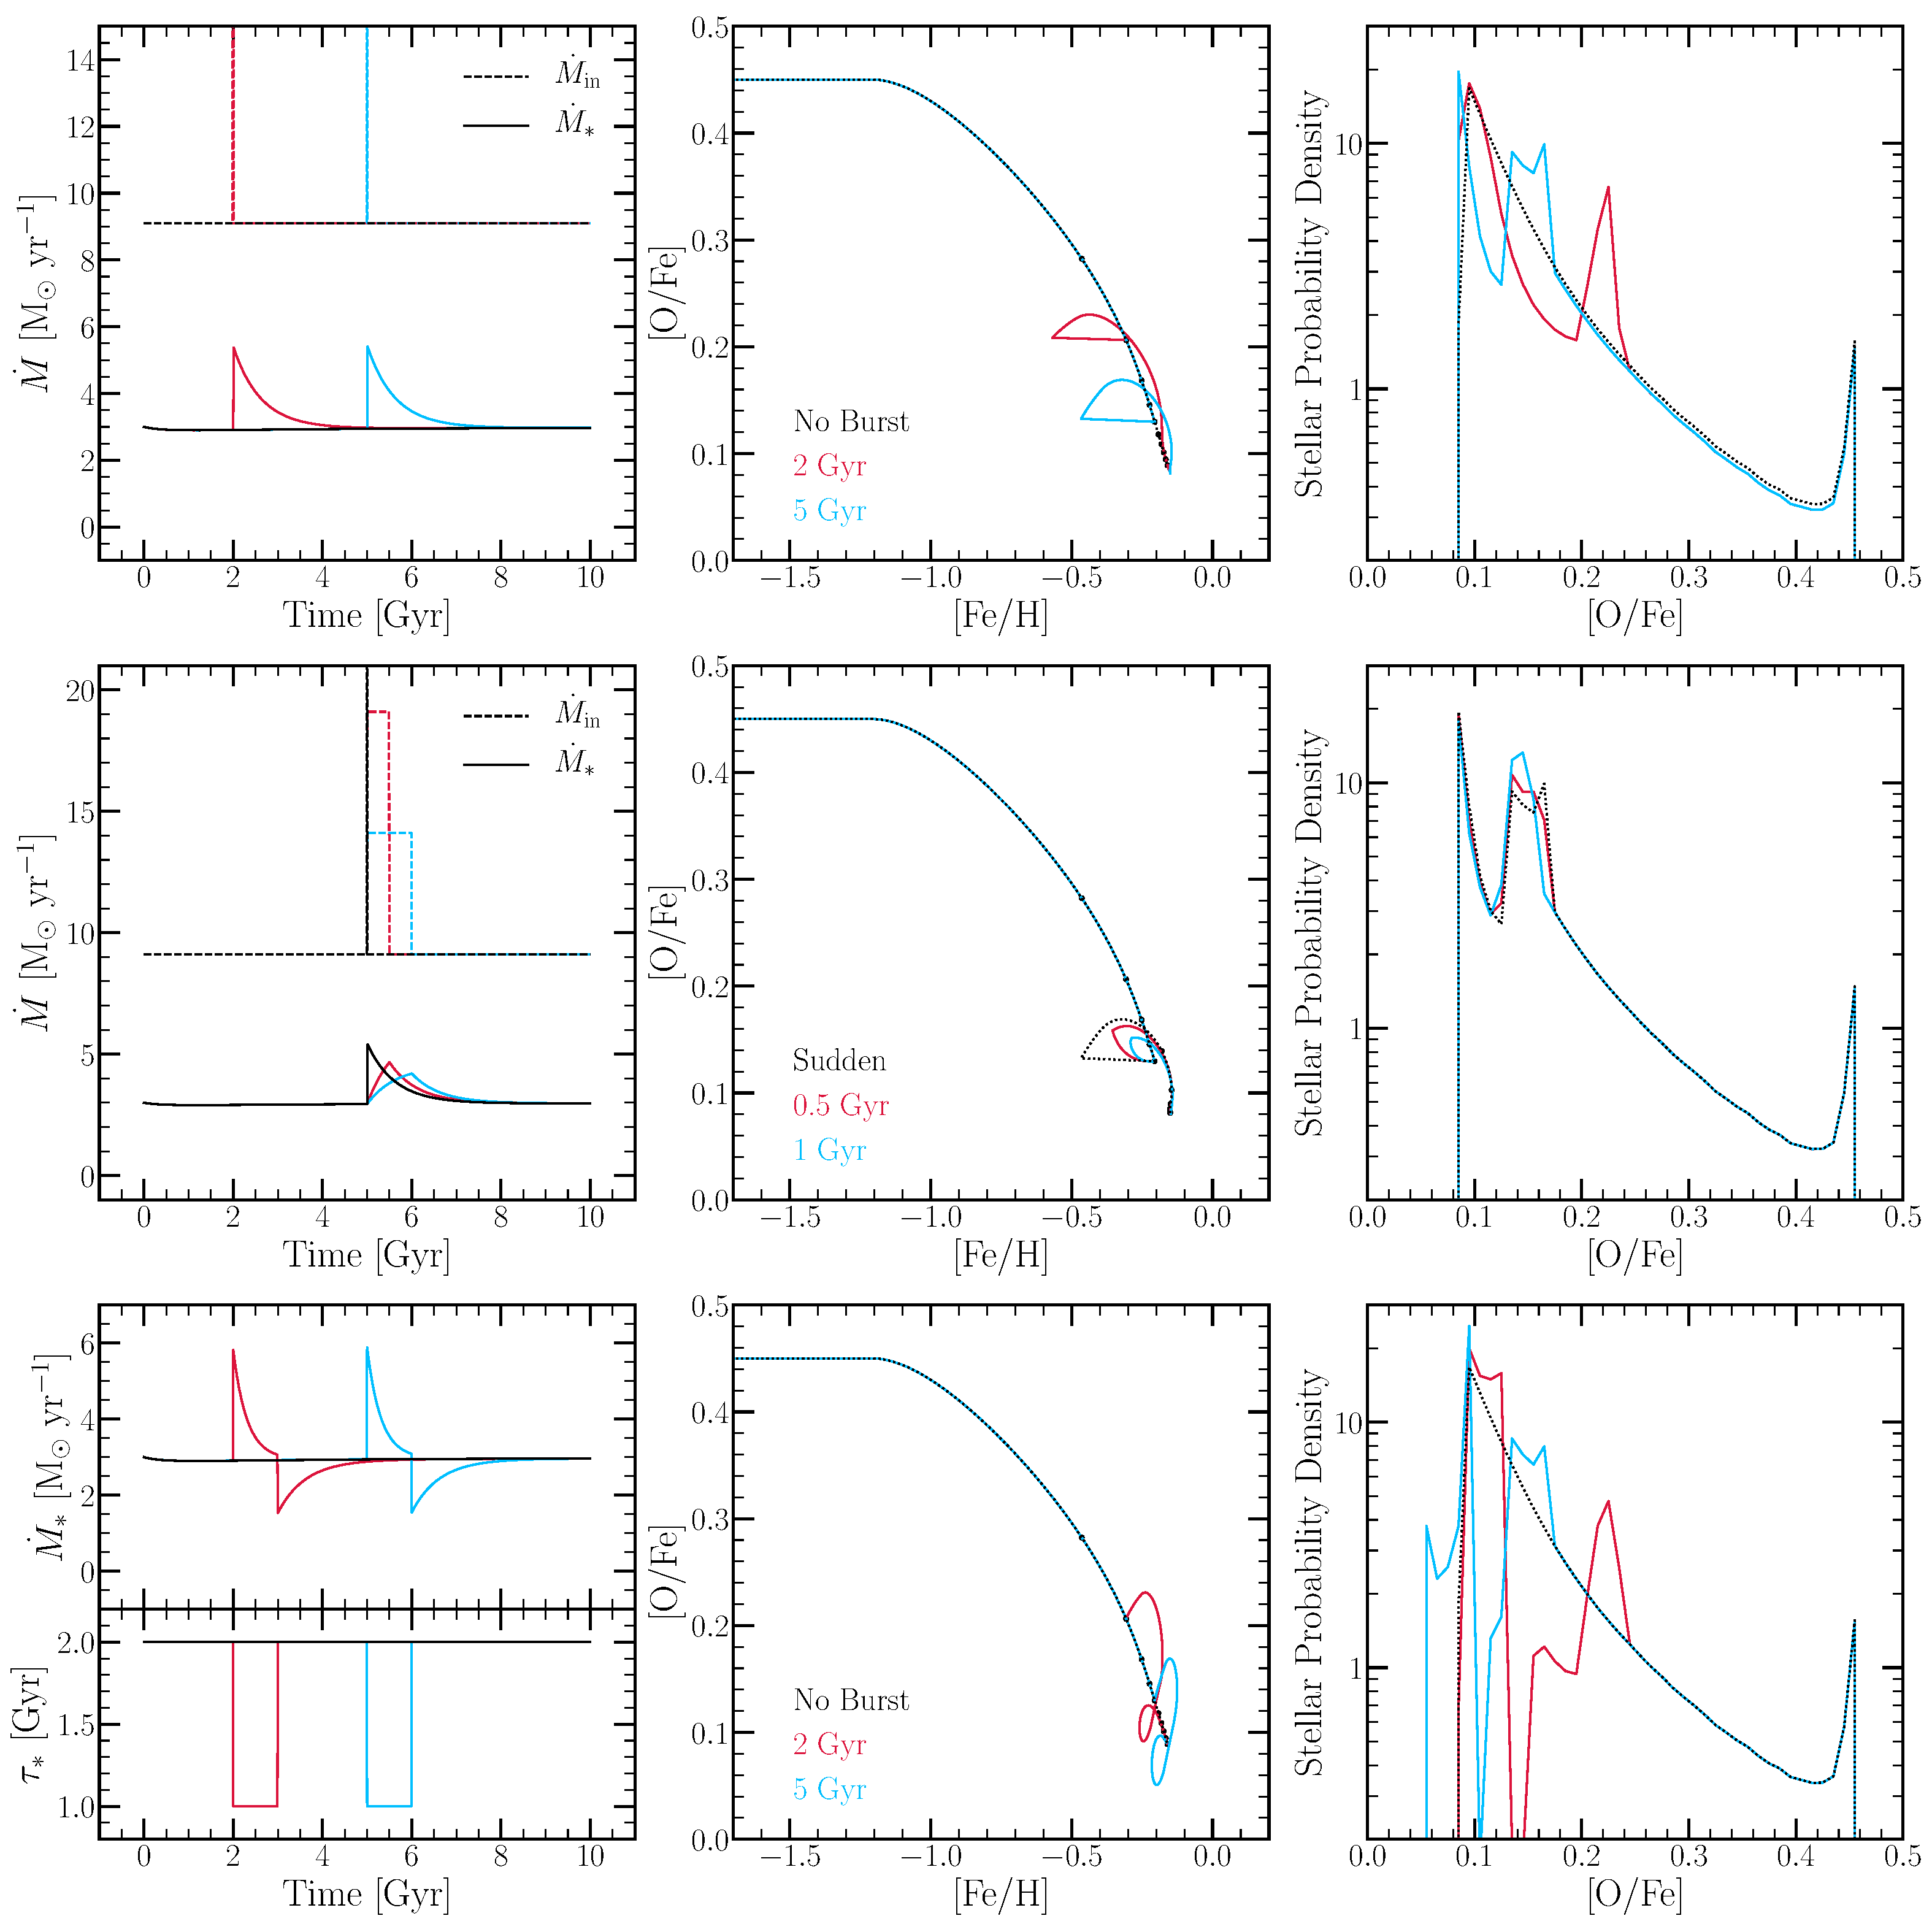
\includegraphics[scale = 0.29]{fiducial_bursts.pdf}
\caption{
Evolutionary tracks in the [O/Fe]-[Fe/H] plane (middle column) and [O/Fe] 
distributions (right column) of starburst GCE models with infall and star 
formation histories shown in left panels. \textbf{Top}: Black curves show an 
unperturbed model with a constant infall rate and near-constant star formation 
rate. Red and blue curves show models with starbursts induced by adding 85\% of 
the ISM mass worth of $Z = 0$ gas at $t = 2$ or $t = 5$ Gyr, 
respectively. \textbf{Middle}: Red and blue curves show models in which the 
gas infall rate is boosted over a time interval of $\Delta t$ = 0.5 Gyr or 1 
Gyr, respectively, at $t = 5$ Gyr. Black curves show the sudden gas infall 
model from the upper row for comparison. The total amount of gas added is the 
same in all three models. \textbf{Bottom}: Red and blue curves show models with 
starbursts induced by doubling the SFE (halving $\tau_*$) for an interval of 
$\Delta t = 1$ Gyr at $t = 2$ Gyr or 5 Gyr, respectively, with the infall rate 
(not plotted) held constant. Black curves show the unperturbed model. In the 
middle panels, small points on the unperturbed model curve mark 1 Gyr 
intervals. 
}
\label{bursts:fig:fiducial_cases}
\end{figure*}

\afterpage{
\clearpage
\begin{landscape}
\begin{figure*} % fig 2
\centering
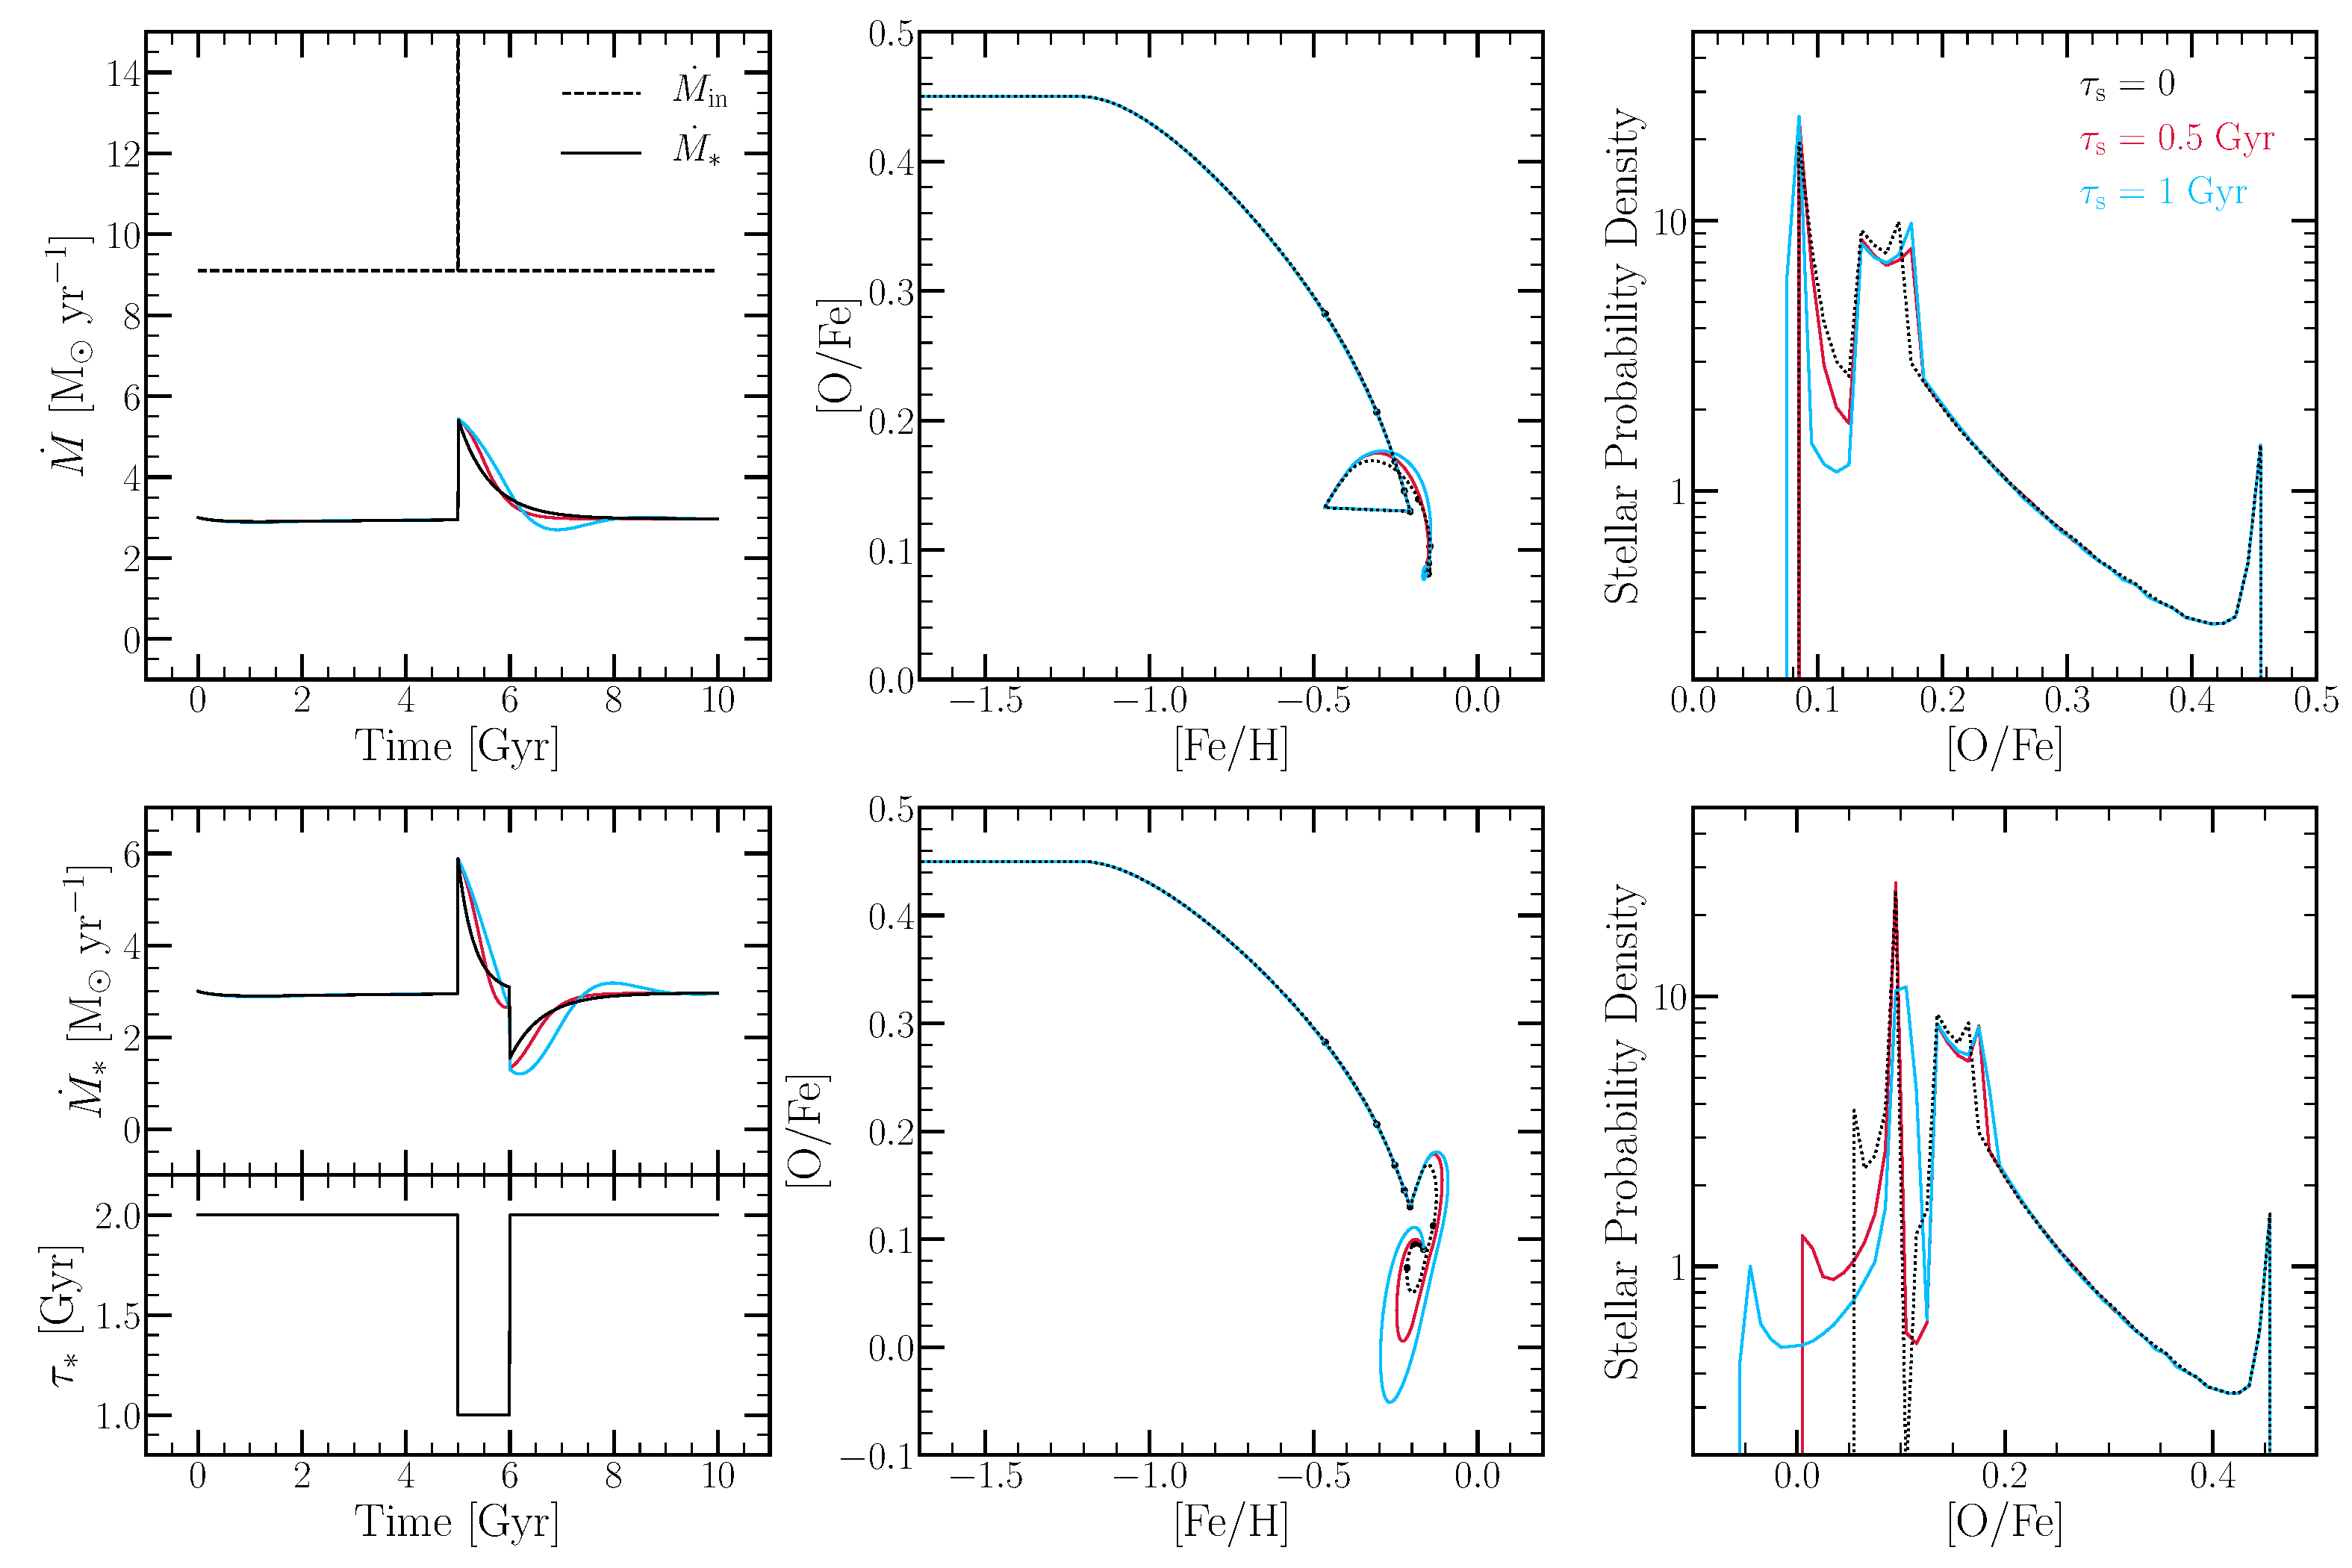
\includegraphics[scale = 0.35]{smoothing_time.pdf}
\caption{
Similar to Fig.~\ref{bursts:fig:fiducial_cases}, for models in which the outflow 
$\dot{M}_\text{out} = \eta\langle\dot{M}_*\rangle_{\tau_\text{s}}$ responds 
to the SFR averaged over a preceding interval $\tau_\text{s} = 0.5$ Gyr (red) 
or 1 Gyr (blue). Top and bottom rows show models in which the starburst is 
induced by increasing the gas supply or SFE, respectively, at $t = 5$ Gyr, as 
in the top and bottom rows of Fig.~\ref{bursts:fig:fiducial_cases}. Black dotted 
curves show the corresponding $\tau_\text{s} = 0$ models, repeated from 
Fig.~\ref{bursts:fig:fiducial_cases}, with small dots at 1 Gyr intervals in the 
middle panels.  
}
\label{bursts:fig:ts_combined}
\end{figure*}
\end{landscape}
\clearpage
}

We begin by defining a GCE model with nearly constant star formation, which we 
will then perturb in a variety of ways. Our fiducial no-burst model has an 
infall rate of $\dot{M}_\text{in} = 9.1\ M_\odot\ \text{yr}^{-1}$ onto a galaxy 
with an initial gas supply of $M_\text{g} = 6.0\times10^9\ M_\odot$, an SFE 
timescale of $\tau_*$ = 2 Gyr, a mass-loading factor of $\eta$ = 2.5, 
$\tau_\text{s}$ = 0, and $\xi_\text{enh}$ = 1 (i.e. Z$_\text{out}$ = 
Z$_\text{gas}$) with continuous recycling. We also adopt a power-law SN Ia 
delay-time distribution (DTD) with R$_\text{Ia} \propto t^{-1.1}$ and minimum 
delay time of $t_\text{D}$ = 150 Myr. In short, this is a model with a 
constant infall rate and (nearly) constant star formation rate with parameters 
that do not change with time. The analytic model of~\citet{Weinberg2017b} 
accurately describes the [O/Fe] evolution of this numerical model. Although we 
adopt explicit numerical values for the initial gas mass and 
$\dot{M}_\text{in}$, the [Fe/H] and [O/Fe] evolution would be unchanged if we 
multiplied both of these quantities by the same constant factor. As shown 
by~\citet{Weinberg2017b}, the characteristic time for the evolution of O 
or other CCSN elements in such a model is the depletion time 
$\tau_\text{dep} \equiv \tau_*/(1 + \eta - r_\text{inst})$, while for Fe the 
evolutionary timescale depends on both $\tau_\text{dep}$ and the characteristic 
SN Ia timescale $\tau_\text{Ia}\sim 1-2$ Gyr. 

\subsection{Gas-Driven Starbursts}
\label{bursts:sec:gas-driven}

\afterpage{
\clearpage
\begin{landscape}
\begin{figure*} % fig 3
\centering
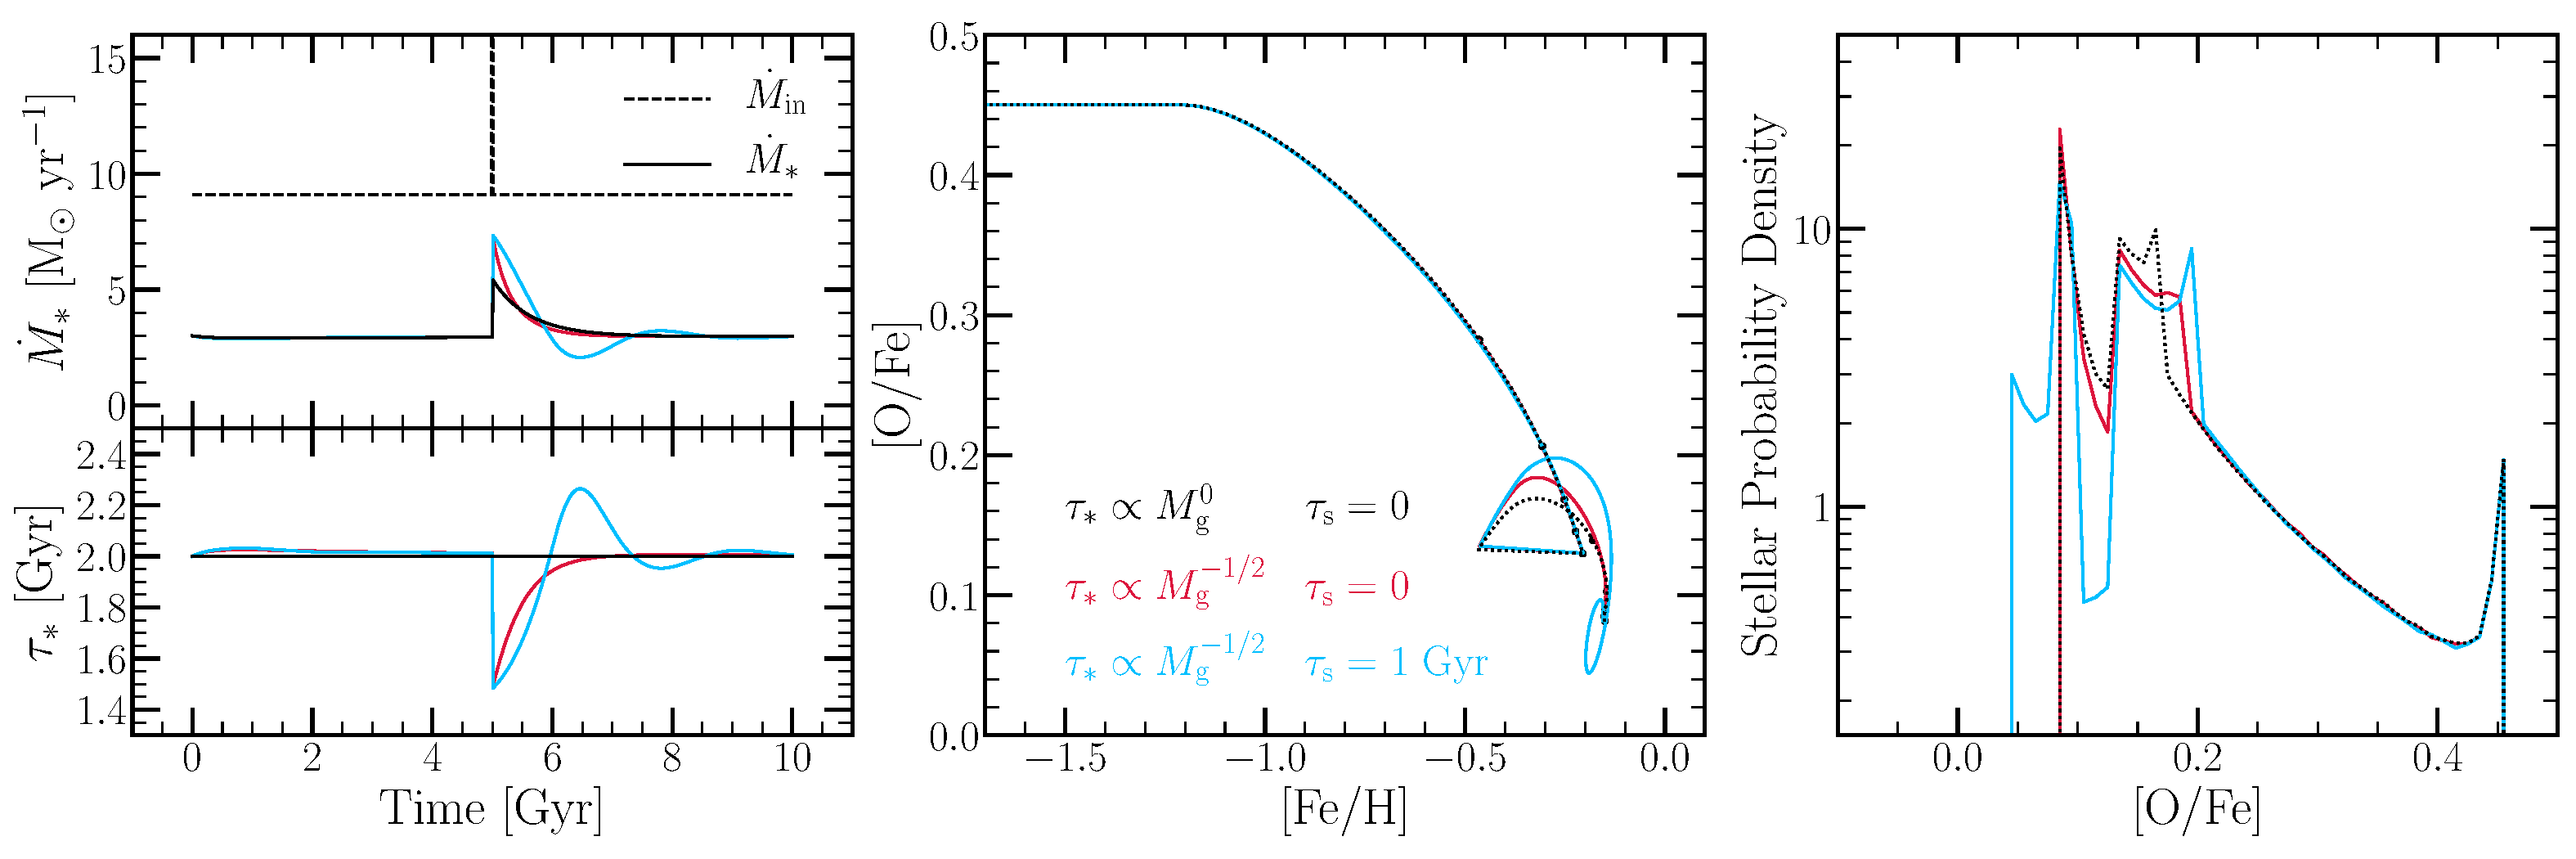
\includegraphics[scale = 0.35]{schmidt_smoothing.pdf}
\caption{
Similar to Fig.~\ref{bursts:fig:fiducial_cases}, for models in which the gas supply 
increases suddenly at $t = 5$ Gyr and the SFE timescale remains constant 
(black dotted) or decreases in accordance with the Kennicutt-Schmidt law (red, 
blue). The blue curve model has smoothing timescale $\tau_\text{s} = 1$ Gyr, 
and the black curve model is identical to the $t = 5$ Gyr starburst in the top 
row of Fig.~\ref{bursts:fig:fiducial_cases}. The lower left panel shows the response 
of $\tau_*$ to the evolving gas supply. 
}
\label{bursts:fig:ts_bolus_schmidt}
\end{figure*}
\end{landscape}
\clearpage
}

Our simplest starburst model is one in which a large amount of gas with a 
specified metallicity is added to the galaxy in a short amount of time. Here 
``large'' means that the added gas is significant compared to the current gas 
supply and ``short'' is relative to the timescales associated with GCE, in 
particular the depletion time $\tau_\text{dep}$. In this paper, we adopt the 
simplest scenario in which the added gas has zero metallicity, but any value 
can be used in \texttt{VICE}. 
\par
The top row of Fig.~\ref{bursts:fig:fiducial_cases} compares two gas-driven 
starburst models to our burstless scenario. These models have the same 
parameters as the burstless scenario with the exception of the infall rate. In 
these models, the infall rate assumes a value of $\dot{M}_\text{in}$ = 5000\ 
$M_\odot \text{yr}^{-1}$ for one $\Delta t$ = 1 Myr timestep, thereby adding 
$\dot{M}_\text{in}\Delta t = 5\times10^9 M_\odot$ of zero metallicity gas 
essentially instantaneously. Red and blue curves show models with gas added at 
$t = 2$ and $5$ Gyr, respectively. In each case, the nearly doubled gas supply 
causes a near doubling of the star formation rate (SFR). This burst decays on 
a timescale of~$\sim$1 Gyr as the excess gas is consumed by star formation and 
outflows. 
\par
The evolution of these models in [O/Fe] vs. [Fe/H] exhibits a ``jump-and-hook'' 
trajectory. Dilution by pristine gas causes an instantaneous jump to lower 
[Fe/H] at fixed [O/Fe]. The burst of star formation elevates the rate of CCSN 
enrichment to SN Ia enrichment, so the ISM evolves to higher [O/Fe] as the 
metallicity increases. Eventually the impact of the starburst dies away and 
the [O/Fe] evolution returns to that of the unperturbed model. 
\par 
The top right panel shows the normalized distribution of [O/Fe] in these 
models. The unperturbed model has two peaks in this distribution, the first at 
[O/Fe] $\approx$ +0.45 for stars formed early in the model galaxy's evolution 
when SN Ia enrichment is still negligible, and the second at 
[O/Fe] $\approx$ +0.08 produced when the system has reached equilibrium and is 
forming stars at constant [Fe/H] and [O/Fe]. For our adopted yields, a constant 
SFR model evolves to slightly super-solar [O/Fe], but a mildly declining SFR 
model would evolve to solar [O/Fe]~\citep[see][figure 3]{Weinberg2017b}. A 
declining SFR would also boost the equilibrium [Fe/H] to solar instead of 
mildly sub-solar for our adopted yields and $\eta$. We have chosen to focus on 
perturbations of a constant SFR model for simplicity, but we have checked that 
our qualitative conclusions hold if the underlying model has exponentially 
declining star formation with $\tau_\text{sfh}\approx$ 6 Gyr. 
\par 
The starburst models produce a third peak in this distribution at intermediate 
values of [O/Fe]. The lower edge of this peak corresponds to the value of 
[O/Fe] at the start of the burst, and the upper edge corresponds to the value 
of [O/Fe] at the top of the hook seen in the middle panel. The peak arises both 
because the system spends extra time at these [O/Fe] values and because the 
SFR is elevated during this time. Although the jump-and-hook trajectories are 
similar for the two starburst models, the arc in [O/Fe] is flatter for the 
earlier burst, which corresponds to a narrower peak in [O/Fe]. This difference 
arises because at $t$ = 2 Gyr the CCSN/SN Ia ratio of the unperturbed model is 
still elevated compared to its eventual equilibrium ratio, so the extra boost 
from the starburst has a smaller relative impact. 
\par 
A gas rich merger or violent dynamical disturbance may induce a very rapid 
increase in a galaxy's supply of star-forming gas. However, a temporary boost 
in a galaxy's gas accretion rate can also induce elevated star formation. 
The middle row of Fig.~\ref{bursts:fig:fiducial_cases} compares the $t = 5$ Gyr 
instantaneous gas increase model to models in which the same 
$5\times10^9 M_\odot$ of gas is added over $\Delta t$ = 0.5 and 1.0 Gyr 
intervals. The perturbation to the SFR is smoother (left panel), though the 
number of ``extra'' stars formed is similar. The hooks in [O/Fe]-[Fe/H] are no 
longer flat-bottomed because the elevated SFR increases [O/Fe] at the same 
time that the infall dilutes [Fe/H]. For $\Delta t$ = 1 Gyr the jump in [O/Fe] 
is small because the maximum boost of SFR is only about half that of the 
instantaneous model. However, the extra peak in the [O/Fe] distribution is 
remarkably similar in all three models, though slightly sharper for 
$\Delta t$ = 1 Gyr. 
Although their model differs in detail, these findings are in good qualitative 
agreement with the ``two-infall'' model predictions presented 
in~\citet{Spitoni2019}. 
\par 
We conclude that a third peak in the [O/Fe] distribution is the characteristic 
observable signature of a gas-driven starburst that formed a significant 
fraction of a system's stars. The location of the peak indicates the value of 
[O/Fe] at the time of the burst. Resolving these peaks requires a large sample 
of stars with precise [O/Fe] (or [$\alpha$/Fe]) values, i.e. statistical errors 
of 0.05 dex or below. Correlating these [$\alpha$/Fe] measurements with 
individual stellar age estimates could increase the diagnostic power even if 
the age estimates have substantial statistical errors. 


\subsection{Efficiency-Driven Starbursts}
\label{bursts:sec:efficiency-driven}
The bottom row of Fig.~\ref{bursts:fig:fiducial_cases} shows a scenario in which 
starbursts arise from a temporary increase of SFE instead of an increase in 
gas supply. We double the SFE -- thus decreasing the SFE timescale $\tau_*$ 
from 2 Gyr to 1 Gyr -- for a period of $\Delta t$ = 1 Gyr, beginning at $t = 2$ 
or 5 Gyr. The gas infall rate is held constant. As in the gas-doubling 
scenario, the SFR initially jumps by a factor of two, then decays to its 
original value. However, once $\tau_*$ returns to 2 Gyr, the SFR drops 
\textit{below} that of the unperturbed model because the gas supply has been 
depleted during the high SFE phase. Over an interval of~$\sim$1 Gyr, the SFR 
recovers to the value of $\dot{M}_*\approx3\ M_\odot\ \text{yr}^{-1}$ at which 
star formation and outflow balance infall. 
\par 
The hooks in [O/Fe]-[Fe/H] evolution have a different morphology for the 
efficiency-driven bursts. Because there is no dilution by low metallicity gas, 
the tracks jump up to higher [O/Fe] with slightly increasing [Fe/H], instead 
of first moving back to lower [Fe/H]. Furthermore, because of the depression 
in SFR once $\tau_*$ returns to its baseline value, the [O/Fe] track dips 
below that of the unperturbed model before returning to it at late 
times. During the downward loop, the rate of SNe Ia is high because of the 
stars formed during the recent burst, but the rate of CCSNe is low due to the 
reduced SFR. 
\par 
The distribution of [O/Fe] in these models again shows an extra peak at [O/Fe] 
values close to those at the onset of the starburst. However, the morphology 
of these distributions is different from that of the gas-driven starburst 
models in two ways. First, the peak in [O/Fe] is followed by a much deeper 
trough at slightly lower [O/Fe] because the SFR is depressed while the ISM is 
evolving through this abundance ratio. Second, the [O/Fe] distribution 
acquires an additional peak at a value that corresponds to the bottom of the 
downward loops in the middle panel. With sufficiently good data, it might be 
possible to distinguish the signature of gas-driven and efficiency-driven 
starbursts from the detailed shape of the [O/Fe] distribution. In particular, 
an efficiency-driven burst at relatively late times would produce a population 
of roughly coeval stars with [$\alpha$/Fe] values below that of the bulk 
population. There is some hint of such a population in the solar 
neighborhood~\citep{Feuillet2018}. 

\subsection{Outflow Smoothing Time}
\label{bursts:sec:smoothing}
We now examine models in which the outflow rate $\dot{M}_\text{out}$ responds 
to the SFR averaged over a time interval $\tau_\text{s}$ instead of the 
instantaneous SFR. Fig.~\ref{bursts:fig:ts_combined} shows star formation histories, 
[O/Fe]-[Fe/H] tracks, and [O/Fe] distributions for gas-driven and 
efficiency-driven starburst models with $\tau_\text{s}$ = 0, 0.5, and 1 Gyr. 
The $\tau_\text{s}$ = 0 models are identical to the t = 5 Gyr burst models 
shown in the top and bottom rows of Fig.~\ref{bursts:fig:fiducial_cases}. Because 
the enhanced infall models (middle row of Fig.~\ref{bursts:fig:fiducial_cases}) are 
qualitatively similar to the instantaneous gas doubling model (top row), we 
show only this limiting case of a gas-driven starburst in the remainder of the 
paper. 
\par 
For the gas-driven starburst, even a 1 Gyr smoothing time has only a small 
impact on the [O/Fe]-[Fe/H] trajectory and [O/Fe] distribution. Just after the 
accretion event, the SFR in the smoothed models is slightly higher than in the 
$\tau_\text{s}$ = 0 model because the outflow rate is lower, and the hook in 
the evolutionary track therefore reaches slightly higher [O/Fe]. For 
$\tau_\text{s}$ = 1 Gyr, the SFR at $t\approx$ 6 - 8 Gyr dips below the 
3 $M_\odot\ \text{yr}^{-1}$ baseline, because the extra accreted gas has been 
consumed and the outflow rate remains high because of the earlier starburst. 
As a result, the deficit in the [O/Fe] distribution at [O/Fe] $\approx$ +0.1 
is deeper in this model. 
\par 
For the efficiency-driven starburst, smoothing has a larger impact because the 
delayed outflow deepens the depression of SFR after the burst. The downward 
hook of [O/Fe] is therefore substantially deeper even for $\tau_\text{s}$ = 0.5 
Gyr. Smoothing of the outflow response exaggerates the characteristic form of 
an efficiency-driven starburst perturbation and moves the extra peak of the 
[O/Fe] distribution to a lower value. 


\subsection{Hybrid Starbursts}
\label{bursts:sec:hybrid}
If the gas supply of a galaxy increases suddenly, then the SFE may also 
increase because of greater gas self-gravity, more rapid cloud collisions, or 
whatever dynamical disturbance drove the gas increase in the first place. 
Observations provide some evidence for starbursts that are driven by both 
increased gas supply and increased 
SFE~\citep[][and the citations therein]{Kennicutt2012}. 
Fig.~\ref{bursts:fig:ts_bolus_schmidt} shows results for a hybrid model in which a 
doubling of the gas supply is linked to a Kennicutt-Schmidt scaling of the SFE, 
with $\tau_* = (2\text{ Gyr})(M_\text{g}/6\times10^9\ M_\odot)^{-1/2}$ (see 
\S~\ref{bursts:sec:methods}). If the smoothing time $\tau_\text{s}$ = 0, then the 
evolution of this hybrid model is only slightly different from that of our 
standard gas-driven starburst, as one can see by comparing the dashed black and 
solid red curves in the middle and right panels of 
Fig.~\ref{bursts:fig:ts_bolus_schmidt}. The hybrid burst has a higher peak SFR, 
which leads to a higher peak of the [O/Fe] hook. For $\tau_\text{s}$ = 1 Gyr, 
the trajectory and [O/Fe] distribution of the hybrid model show features of 
both the gas-driven and efficiency-driven models. In particular, this model 
has a period of depressed SFR because of the delayed ejection of gas by the 
starburst, and the enhanced ratio of SNe Ia/CCSNe during this period causes a 
downward hook in [O/Fe] and an additional peak in the [O/Fe] distribution. 

